\section{Evaluating Mechanical Energy Conservation}

\begin{figure}[h]
	\centering
	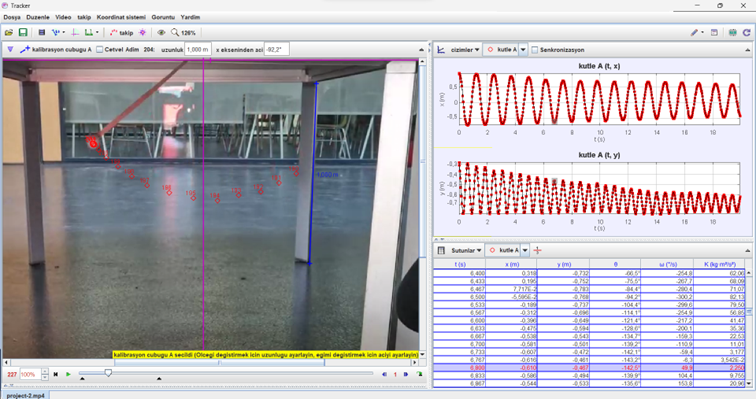
\includegraphics[width=1\textwidth]{assets/experiment.png}
	\caption{Experiment Calculations - \url{https://youtu.be/ML8BPKV-HQA}}
\end{figure}

Our experimental data revealed the following trend in mechanical energy ($E$) of the pendulum across several oscillation cycles:

\begin{table}[h]
	\centering
	\begin{tabular}{l|c|r}
		\textbf{Time} & \textbf{Mechanical Energy} & \textbf{Percentage Loss} \\
		\hline
		$t_{1}$ & $135kJ$ & $0\%$\\
		$t_{2}$ & $118kJ$ & $12.6\%$\\
		$t_{3}$ & $103kJ$ & $23.7\%$\\
		$t_{4}$ & $96kJ$ & $28.9\%$\\
		$t_{5}$ & $87kJ$ & $35.6\%$\\
		$t_{6}$ & $80kJ$ & $40.7\%$\\
		$t_{7}$ & $71kJ$ & $47.4\%$\\
	\end{tabular}
	\caption{Mechanical Energy of the Pendulum}
\end{table}

\newpage
\thispagestyle{plain}

As we can observe, the mechanical energy is not perfectly conserved throughout the oscillations. We see a gradual decrease in $E$ from $135kJ$ at $t_{1}$ to $71kJ$ at $t_{7}$, representing a total loss of approximately $47\%$ over the observed time-frame.

This decline in energy aligns with our expectations for a real-world pendulum due to the presence of dissipative forces like:

\begin{itemize}
	\item \textbf{Air resistance:} Friction with the surrounding air continually extracts energy from the system, slowing down the oscillations and reducing the amplitude.
	\item \textbf{Joint resistance:} Friction at the pivot point also dissipates energy as heat and sound, contributing to the decrease in mechanical energy.
\end{itemize}

While the model based on Eq. (3) assumes ideal conditions with no energy loss, our experimental data highlights the impact of these non-ideal factors in real-world scenarios. The observed rate of energy loss provides valuable insights into the magnitude of these dissipative forces and their influence on the pendulum's motion.
